\documentclass{beamer}
\usepackage{amsmath,amssymb,amsthm,slashed, euscript}
\usepackage{graphicx}


\textwidth=110mm


\title{Weak fundamental group of noncommutative $C^*$-algebras}
\institute
{
Algebras in analysis
}

\author{Petr R. Ivankov  }



\theoremstyle{plain}
\newtheorem{defn}{Definition}
\newtheorem{rem}{Remark}
\newtheorem{exm}{Example}
\newtheorem*{claim}{Claim}
\newtheorem{prop}{Proposition}
\newtheorem{empt}[prop]{}%[section]
\newtheorem{lem}{Lemma}%[section]
\newtheorem{thm}{Theorem}%[section]



\newcommand{\A}{\mathcal{A}}
\newcommand{\be}{\begin{equation}}
\newcommand{\ee}{\end{equation}}
\newcommand{\Ga}{\Gamma}
\newcommand{\B}{\mathcal{B}}
\newcommand{\Cc}{\mathcal{C}}
\newcommand{\C}{\mathbb{C}}
\newcommand{\D}{\mathcal{D}}
\newcommand{\G}{\mathcal{G}}
\newcommand{\Hc}{\mathcal{H}}
\newcommand{\Lc}{\mathcal{L}}
\newcommand{\Pc}{\mathcal{P}}
\newcommand{\Sc}{\mathcal{S}}
\newcommand{\U}{\mathcal{U}}
\newcommand{\rar}{\rightarrow}
\newcommand{\Ef}{\mathbb{E}}
\newcommand{\desc}{\mathfrak{desc}}


%Uppercase Gothic characters
\newcommand{\gtA}{\mathfrak{A}}
\newcommand{\gtB}{\mathfrak{B}}
\newcommand{\gtM}{\mathfrak{M}}
\newcommand{\gtN}{\mathfrak{N}}
\newcommand{\gtP}{\mathfrak{P}}
\newcommand{\gtS}{\mathfrak{S}}

%Lowercase Gothic characters
\newcommand{\gtf}{\mathfrak{f}}
\newcommand{\gtg}{\mathfrak{g}}

%Bold Characters
\newcommand{\Cb}{\mathbb{C}}
\newcommand{\Nb}{\mathbb{N}}
\newcommand{\Rb}{\mathbb{R}}
\newcommand{\Zb}{\mathbb{Z}}

%Uppercase Greek characters
\newcommand{\Gm}{\Gamma}
\newcommand{\Te}{\Theta}
\newcommand{\Om}{\Omega}
\newcommand{\s}{ }

%Lowercase Greek characters
\newcommand{\al}{\alpha}
\newcommand{\gm}{\gamma}
\newcommand{\dl}{\delta}
\newcommand{\sg}{\sigma}
\newcommand{\ph}{\varphi}
\newcommand{\te}{\theta}
\newcommand{\ze}{\zeta}
\newcommand{\lift}{\mathfrak{lift}}

\newcommand{\Id}{\mathrm{Id}}
\newcommand{\Aut}{\mathrm{Aut}}
\newcommand{\Coo}{{\mathrm{C}}^\infty}
\newcommand{\alg}{\mathrm{alg}}
\newcommand{\diag}{\mathrm{diag}}
\newcommand{\spinc}{\textbf{$spin^c$}}
\newcommand{\Hom}{\mathrm{Hom}}
\newcommand{\supp}{\mathrm{supp}}
\newcommand{\Ccl}{\mathbf{C}l}
\newcommand{\xto}{\xrightarrow}

\newcommand{\lto}{\longrightarrow}
\newcommand{\ox}{\otimes}
\newcommand{\nb}{\nabla}
\newcommand{\sS}{\mathcal{S}}
\newcommand{\Dn}{D\!\!\!\!/}
%\newcommand{\ij}{{i,j}}
\newcommand{\aC}{\ensuremath{\underline{\Cb}} }
\newcommand{\scp}[2]{\left\langle{#1},{#2}\right\rangle}
\newcommand{\op}[1]{J{#1}J^\dag}
\newcommand{\sA}{\mathcal{A}} 
\newcommand{\sB}{\mathcal{B}}       %%
\newcommand{\sC}{\mathcal{C}}       %%
\newcommand{\sD}{\mathcal{D}}       %%
\newcommand{\sE}{\mathcal{E}}       %%
\newcommand{\sF}{\mathcal{F}}       %%
\newcommand{\sG}{\mathcal{G}}       %%
\newcommand{\sH}{\mathcal{H}}       %%
\newcommand{\sI}{\mathcal{I}}       %%
\newcommand{\sJ}{\mathcal{J}}       %%
\newcommand{\sK}{\mathcal{K}}       %%
\newcommand{\sL}{\mathcal{L}}       %%
\newcommand{\sM}{\mathcal{M}}       %%
\newcommand{\sN}{\mathcal{N}}       %%
\newcommand{\sO}{\mathcal{O}}       %%
\newcommand{\sP}{\mathcal{P}}       %%
\newcommand{\sQ}{\mathcal{Q}}       %%
\newcommand{\sR}{\mathcal{R}}       %%
\newcommand{\sT}{\mathcal{T}}       %%
\newcommand{\sU}{\mathcal{U}}       %%
\newcommand{\sV}{\mathcal{V}}       %%
\newcommand{\sX}{\mathcal{X}}       %%
\newcommand{\sY}{\mathcal{Y}}       %%
\newcommand{\sZ}{\mathcal{Z}}       %%
\newcommand{\N}{\mathbb{N}}                  %% 

\renewcommand{\a}{\alpha}     
\newcommand{\la}{\lambda}     
\newcommand{\La}{\Lambda}
\newcommand{\bt}{\beta}           %% short for  \beta
 
    
\newcommand{\bydef}{\stackrel{\mathrm{def}}{=}}  
\newcommand{\hookto}{\hookrightarrow}        %% abbreviation
  
\begin{document}
%\titlepage
\begin{frame}
  \titlepage
\end{frame}
\begin{frame}

		\begin{figure}
			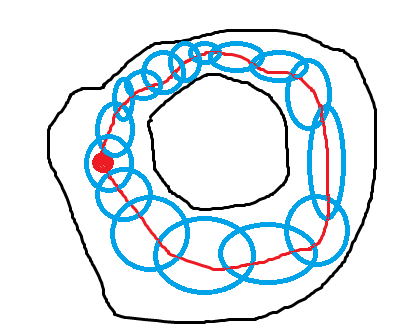
\includegraphics[width=\linewidth]{PICTURE.png}
			\caption{A boat.}
			\label{fig:boat1}
		\end{figure}
		Figure \ref{fig:boat1} shows a boat.
\end{frame}
\begin{frame}
\begin{definition}\label{top_weakly_semi1_defn}\alert{Petr Ivankov.}
		An open connected subset $\sU\subset \sX$ of a topological space is said to be \alert{semilocally proper} it is evenly covered by any covering $p:\widetilde{\sX}\to\sX$, i.e. $p^{-1}\left(\sU \right)$ is a disjoint union of homeomorphic to $\sU$ sets. 
A space $\sX$ is said to be \alert{weakly semilocally 1-connected} if for  every point $x$ and there is a semilocally proper neighborhood.
\end{definition} 
\begin{example}
	Any connected, path connected, locally path connected, semilocally 1-connected   space is weakly semilocally 1-connected.
\end{example}

\end{frame}

\begin{frame}
	\begin{definition}\label{top_weak_path_defn}\alert{Petr Ivankov.}
		Let $\sX$ be a topological space.	A \alert{weak path on} $\sX$ is a finite sequence $\left(\sU_1, ..., \sU_n\right)$ of open  connected subsets of $\sX$ such that $\sU_j \cap \sU_{j+1} \neq \emptyset$ for any $j = 1, ..., n - 1$. A weak path $\left(\sU_1, ..., \sU_n\right)$ is said to be \alert{weakly semilocally 1-connected} if $\sU_j$ is semilocally proper for all $j = 1,..., n$.
	\end{definition}
		There is an involution * on the set of paths such that
\be\label{top_path_inv_eqn}
\left(\sU_{1},...,\sU_{n}\right)^*\bydef \left(\sU_{n},...,\sU_{1}\right).
\ee
\begin{definition}\label{top_path_comp_defn}\alert{Petr Ivankov.}
	If both $\mathfrak p'=\left(\sU'_{1},...,\sU'_{k}\right)$ and $\mathfrak p''=\left(\sU''_{1},...,\sU_{l}''\right)$ are paths such that $\sU'_{k} \cap \sU''_{1}\neq\emptyset$ then we say that a pair $\left( \mathfrak p', \mathfrak p''\right)$ is \alert{composable}, and the path $\mathfrak p=\left(\sU'_{1},...,\sU'_{k},\sU''_{_1},...,\sU_{l}'' \right)$  is said to be the \alert{composition} of $\mathfrak p'$ and $\mathfrak p''$. We write
\be\label{top_path_comp_eqn}
\mathfrak p'\circ \mathfrak p''\bydef\mathfrak p.
\ee
\end{definition}
	
\end{frame}
\begin{frame} \alert{Petr Ivankov.}
	
		The composition is associative, i.e.  if both pairs $\left( \mathfrak p', \mathfrak p''\right)$ and $\left( \mathfrak p'', \mathfrak p'''\right)$ are composable then one has
	\be\label{top_path_ass_eqn}
	\left( \mathfrak p'\circ \mathfrak p''\right)  \circ \mathfrak p''' = \mathfrak p'\circ \left( \mathfrak p'' \circ \mathfrak p'''\right) .
	\ee 
	If $p: \widetilde{\sX} \to \sX$ is a covering and $\widetilde{\mathfrak p}\bydef \left(\widetilde\sU_1, ..., \widetilde\sU_n\right)$ is weak path on $\widetilde\sX$ then $\mathfrak p\bydef \left(p\left( \widetilde\sU_1\right) , ..., p\left( \widetilde\sU_n\right) \right)$ is a weak path on $\sX$.
		\begin{definition}\label{top_path_desc_defn}
		In the above situation we say that $\mathfrak p$ is a $p$-\alert{descent} of $\widetilde{\mathfrak p}$. We write
		\be\label{top_path_desc_eqn}
		\mathfrak p\bydef \desc_p\left( \widetilde{\mathfrak p}\right). 
		\ee
	\end{definition}
	
	\end{frame}

\begin{frame}


\begin{definition}\label{top_gen_path_defn}\alert{Petr Ivankov.}
	Let $\sX$ be a connected, locally connected, locally compact, Hausdorff space.
	Let $\mathfrak{A}\bydef\left\{\sU_\a\right\}_{\a \in \mathcal A}$ be a family of connected open subsets of $\sX$, such that $\sX = \cup~ \sU_\a$ and  a closure of $\sU_\a$ is compact for all $\a\in \mathcal A$. A weak path $\left(\sU_{\a_1},...,\sU_{\a_n}\right)$ (cf. Definition \ref{top_weak_path_defn}) on $\sX$  is said to be an  $\mathfrak{A}$-\textit{path} if  $\sU_j \in \mathfrak{A}$ for all $j = 1,...,n-1$.
\end{definition}
\begin{lemma}\label{top_gen_path_lem}	\alert{P. Ivankov}.
	Consider the situation of the above Definition. For any $\sU_{\a'}, \sU_{\a''} \in \mathfrak{A}$ there is a $\left\{\sU_\a\right\}$-{path} $\left(\sU_{\a_1},...,\sU_{\a_n}\right)$ such that $\sU_{\a_1}=\sU_{\a'}$ and $\sU_{\a_n}=\sU_{\a''}$ .
\end{lemma}

\end{frame}
\begin{frame}
	\begin{defn}\label{top_closed_path_defn}	\alert{P. Ivankov}.
		If $\left(\sX, x_0\right)$ is a pointed space then a path $\left(\sU_1, ..., \sU_n\right)$ on $\sX$ is said to be $x_0$-\alert{path} if $x_0\in\sU_1$.  An  $x_0$-{path} is said to be \alert{closed} if $x_0\in\sU_n$.
	\end{defn}
Any pair of closed path is composable.
\begin{lemma}\alert{P. Ivankov}.
	Let $p: \left(\widetilde\sX, \widetilde x_0\right)\to\left(\sX, x_0\right)$ be a pointed covering, and let $\mathfrak{A}\bydef\left\{\sU_\a\right\}_{\a \in \mathcal A}$ 
be a family of connected all open subsets of $\sX$ evenly covered by $p$. Let  ${\mathfrak p}\bydef \left(\sU_1, ..., \sU_n\right)$ be a $\mathfrak{A}$-{path}, such that $x_0\in\sU_1$. There is an unique  $\widetilde{\mathfrak p}\bydef \left(\widetilde \sU_1, ...,\widetilde \sU_n\right)$ such that $\widetilde x_0 \in \widetilde \sU_1$ and ${\mathfrak p}$ is the $p$-descent of $\widetilde{\mathfrak p}$.
\end{lemma}	
\begin{definition}\label{top_path_lift_defn}\alert{P. Ivankov}.
	The given by the above path $\widetilde{\mathfrak p}$ is said to be the $p$-\alert{lift} of $\mathfrak p$. We write
	\be\label{top_path_lift_eqn}
	\lift_p~\mathfrak p\bydef\widetilde{\mathfrak p}.
	\ee 
\end{definition}
\end{frame}
\begin{frame}
\begin{definition}\label{top_contactible_path_defn}\alert{P. Ivankov}
	Let 
	$\left(\sX, x_0\right)$ be  a pointed space such that  $\sX$ is a connected, locally connected and weakly semilocally 1-connected space.  A closed  semilocally 1-connected path $x_0$-path $\left(\sU_1, ..., \sU_n\right)$ is said to be \alert{contractible} if for any pointed covering  $p: \left(\widetilde\sX, \widetilde x_0\right)\to\left(\sX, x_0\right)$ a $p$-{lift} of $\mathfrak p$ is closed.
\end{definition}
If $\mathfrak p$ is a closed semilocally 1-connected $x_0$-path then both compositions $\mathfrak p^* \circ \mathfrak p$ and $\mathfrak p \circ \mathfrak p^*$ are contractible.
\end{frame}

\begin{frame}
\begin{definition}\alert{P. Ivankov}.
	We say that both closed, weakly semilocally 1-connected  $x_0$-paths $\mathfrak p_1$ and $\mathfrak p_2$ are \textit{homotopically equivalent} if a composition $\mathfrak p_1 \circ \mathfrak p^*_2$ is contractible.
\end{definition}
From our construction it follows that the set of classes of closed weakly semilocally 1-connected $x_0$-paths modulo homotopical equivalence  is a group with  a composition  and an inversion given by $\circ$ and $*$ operations respectively.
\begin{definition}\label{top_weak_fundamental_group_defn}\alert{P. Ivankov}.
	If
	$\left(\sX, x_0\right)$ is  a pointed space, such that $\sX$ is a connected, locally connected and weakly semilocally 1-connected space
	then the described above group is said to be a \alert{weak fundamental group} of $\sX$. We denote it by $\pi_1^{\mathrm{w}}\left(\sX, x_0 \right) $.
\end{definition}

\end{frame}
\begin{frame}
	\begin{lemma}\alert{P. Ivankov}.
\label{top_fundamental_group_mor_exer}
	Let  $p: \left( \widetilde{\sX}, \widetilde{x}_0\right) \to \left(\sX, x_0\right)$ be a pointed covering such that $\sX$ is a connected, locally connected and weakly semilocally 1-connected space. The $p$-descent yields an injective homomorphism $\pi_1^{\mathrm{w}}\left(p \right): \pi_1^{\mathrm{w}}\left(\widetilde\sX, \widetilde x_0 \right)\hookto \pi_1^{\mathrm{w}}\left(\sX, x_0 \right)$. 
\end{lemma}
\begin{lemma}\alert{P. Ivankov}.
	If $\sX$ be a connected, locally path-connected  and  semilocally 1-connected  space. then there is a natural isomorphism
\be
\pi_1^{\mathrm{w}}\left(\sX, x_0 \right)\cong \pi_1\left(\sX, x_0 \right)
\ee
between the weak fundamental group, and the classical one.

\end{lemma}
\end{frame}
\begin{frame}
Let $\left(\sX, x_0\right)$ be  a pointed space, such that $\sX$ is a connected, locally connected and weakly semilocally 1-connected space. 
For any $x \in \sX$ denote by $\mathfrak{Paths} \left( x_0, x\right)$ a set of all semilocally 1-connected $x_0$-paths such that $$
\left( \sU_1, ..., \sU_n\right)\in \mathfrak{Paths} \left( x_0, x\right) \quad \Leftrightarrow \quad x_0 \in \sU_1 \quad x \in \sU_n.
$$
There is an equivalence relation $\sim_{\left( x_0, x\right)}$ on $\mathfrak{Paths} \left( x_0, x\right)$ such that
$$
\mathfrak p_1, \mathfrak p_2 \in  \mathfrak{Paths} \left( x_0, x\right)~~ \mathfrak p_1\sim_{\left( x_0, x\right)} \mathfrak p_2 ~~\Leftrightarrow ~~ \mathfrak p^*_1\circ  \mathfrak p_2 \text{ is contractible (cf. Definition \ref{top_contactible_path_defn})}.
$$
A class of equivalence of $\mathfrak p \in \mathfrak{Paths} \left( x_0, x\right)$ will be denoted by $$\left[\mathfrak p\right]_{\left( x_0, x\right)}\in \mathfrak{Paths} \left( x_0, x\right)/\sim_{\left( x_0, x\right)}.$$
Let $\widetilde \sX$ be a set of pairs $\left(x, \left[\mathfrak p\right]_{\left( x_0, x\right)}\right)$ where $$\left[\mathfrak p\right]_{\left( x_0, x\right)}\in  \mathfrak{Paths} \left( x_0, x\right)/\sim_{\left( x_0, x\right)}.$$ There is a natural map 
\be
\begin{split}
	\widetilde p: \widetilde \sX\to \sX,\\
	\left(x, \left[\mathfrak p\right]_{\left( x_0, x\right)}\right)\mapsto x.
\end{split}
\ee
\end{frame}
\begin{frame}
For any $\mathfrak p = \left( \sU_1, ..., \sU_n\right)\in \mathfrak{Paths} \left( x_0, x\right)$ we define a set 
\be\label{top_u_path_eqn}
\widetilde \sU_{\mathfrak p} \bydef \left\{\left.  \left( x',  \left[\mathfrak p\right]_{\left( x_0, x'\right)}\right)\in \widetilde{\sX} \right|x' \in \sU_n\right\}.
\ee
\begin{thm}\label{top_uni_top_lem}
	If $\sX$ is a connected,  weakly semilocally 1-connected then one has:
	\begin{itemize}
		\item a family of sets given by the equation \eqref{top_u_path_eqn} a {basis} for a topology on $\widetilde\sX$ such that,
		\item the natural map  	$\widetilde p: \widetilde \sX\to \sX$ is an universal covering. 
	\end{itemize}
\end{thm}
\begin{lemma}\label{top_weak_covering_iso_exer}
	Let $\left(\sX, x_0\right)$ be  a pointed space, such that $\sX$ is a connected, locally connected and weakly semilocally 1-connected space, and let $p: \widetilde\sX\to\sX$ be an universal covering. There is a following natural isomorphism
	$$
	\pi^{\text{w}}_1\left(\sX, x_0\right)\cong G\left(\left. \widetilde \sX\right|\sX \right)  
	$$
	where  $G\left(\left. \widetilde \sX\right|\sX \right)$ is a group of covering transformations. 
	
\end{lemma}


\end{frame}
\begin{frame}
		Let $I^2_o = \left[0,1\right]^2$ be a unit square. We order $I^2_o$ lexicographically, i.e.
	$$
	\forall (x, y),(u, w) \in \left[0,1\right]^2 = I^2_o \quad (x, y)< (u, w)  = \begin{cases}
		y < w & x = u\\
		x < u & \text{otherwise}
	\end{cases}
	$$
	and place the order topology on $I^2_o$. It is known that $I^2_o$ is connected but it is not path connected.
	The space $I^2_o$ is said to be the \alert{the ordered square}.
	Let $\sim$ is an equivalence relation on  $I^2_o$ such that $\left(0, 0 \right)\sim \left(1, 1 \right)$ and denote by $\sX \bydef I^2_o/\sim$.
	\begin{lemma}
	If $x_0 \bydef \left(0, 0 \right)/\sim$ then there ia an isomorphism  $	\pi^{\text{w}}_1\left(\sX, x_0\right)\cong\mathbb{Z}$.
	\end{lemma}
\end{frame}
\begin{frame}
The weak fundamental group can be defined algebraically. There is a notion of noncommutative fundamental group (cf. https://arxiv.org/abs/1904.13130), such that there is a family $\mathfrak F$ of $C^*$-algebras such that for any $A\in \mathfrak F$ there is a fundamental group $\pi_1\left(A \right)$. 
\begin{theorem}\alert{Petr Ivankov}
If a topological space $X$ is connected, locally connected and weakly semilocally 1-connected then $C_0\left(X \right) \in \mathfrak F$ and there is a natural isomorphism $\pi_1\left( C_0\left(X \right)\right)  \cong \pi^{\text{w}}_1\left(\sX, x_0\right)$.
\end{theorem}
\end{frame}
\end{document}























